% Use Beamer to create presentations with LaTeX.
\documentclass[aspectratio=169,14pt]{beamer}

% Todos os documentos em português deveriam ter isso...
\usepackage[utf8]{inputenc}
\usepackage[brazil]{babel}

% Utilizaremos fontes T1
\usepackage[T1]{fontenc}

% Toda palestra que se preze, inclui gráficos.
\usepackage{graphics}

% Configura a apresentação para ser executada em tela cheia.
%\hypersetup{pdfpagemode=FullScreen}

% Hide beamer navigation simbols
%\beamertemplatenavigationsymbolsempty

%
% Configuração da apresentação.
%

%
% Escolha o tema e as cores.
% Há um catálogo, completo disponível em
%    http://www.deic.uab.es/~iblanes/beamer_gallery/index_by_theme_and_color.html
%
\usetheme{boxes}
\usecolortheme{orchid}

%
% Altere o tema como desejar.
%

% Centraliza os títulos dos slides.
\setbeamertemplate{frametitle}[default][center]

%
% Dados da apresentação
%
\title[Apresentações com o Beamer]{Uma introdução à confecção de apresentações com o
Beamer, baseada em código.}
\subtitle{Porque basear em vídeo é muito \emph{mainstream}...}
\author{Rafael Jeffman}
\institute[Tchelinux]{Tchelinux}
\titlegraphic{
\includegraphics[width=30px]{images/Tuxgaucho.png}}
\date{18/05/2017}

% * Pacote que controlará o posicionamento de overlays na apresentacao.
\usepackage{tikz}

%
% A partir deste ponto, começam os slides da apresentação
%
\begin{document}

%
% Cada slide da apresentação é chamado de "frame".
%

% Slide especial, criado para ser a abertura da apresentação
\begin{frame}
    \titlepage
\end{frame}

% Corrigindo a imagem da página de título.
{%
    % remove o gráfico original.
    \titlegraphic{}
    \begin{frame}
        % Cria um overlay para uma imagem.
        \begin{tikzpicture}[remember picture,overlay]  
            % Posiciona o overlay na página
            \node [xshift=-3cm,yshift=3cm] at (current page.south east)
            % Adiciona a imagem, definindo seu tamanho
            {
\includegraphics[width=4cm]{images/Tuxgaucho.png}};
        \end{tikzpicture}
        
        % dezenha a página após a imagem.
        \titlepage
    \end{frame}
}

% Cria um slide com título e itens
\begin{frame}
    % Definee o título do frame
    \frametitle{Agenda do Dia}
    % Adiciona itens enumerados.
    \begin{enumerate}
        \item{Aprenda}
        \item{Crie}
        \item{Faça}
        \item{Ensine}
    \end{enumerate}
\end{frame}

% Cria um slide com titulo, items e uma imagem.
\begin{frame}
    \frametitle{Títulos são importantes}
    % Adiciona itens sem numeração.    
    \begin{itemize}
        \item{Não utilize muito texto em uma apresentação.}
        \item{\LaTeX\ é feito para se concentrar no conteúdo.}
        \item{Beamer, ainda é \LaTeX.}
    \end{itemize}
        
    % Cria um overlay para uma imagem.
    \begin{tikzpicture}[remember picture,overlay]  
        % Posiciona o overlay na página
        \node [xshift=\paperwidth / 2,yshift=2cm] at (current page.south west)
        % Adiciona a imagem, definindo seu tamanho
        {
\includegraphics[width=2cm]{images/Tuxgaucho.png}};
    \end{tikzpicture}
\end{frame}

% Cria um slide com uma única imagem, definida como imagem de fundo.
{%
    \usebackgroundtemplate{
        %\centering
        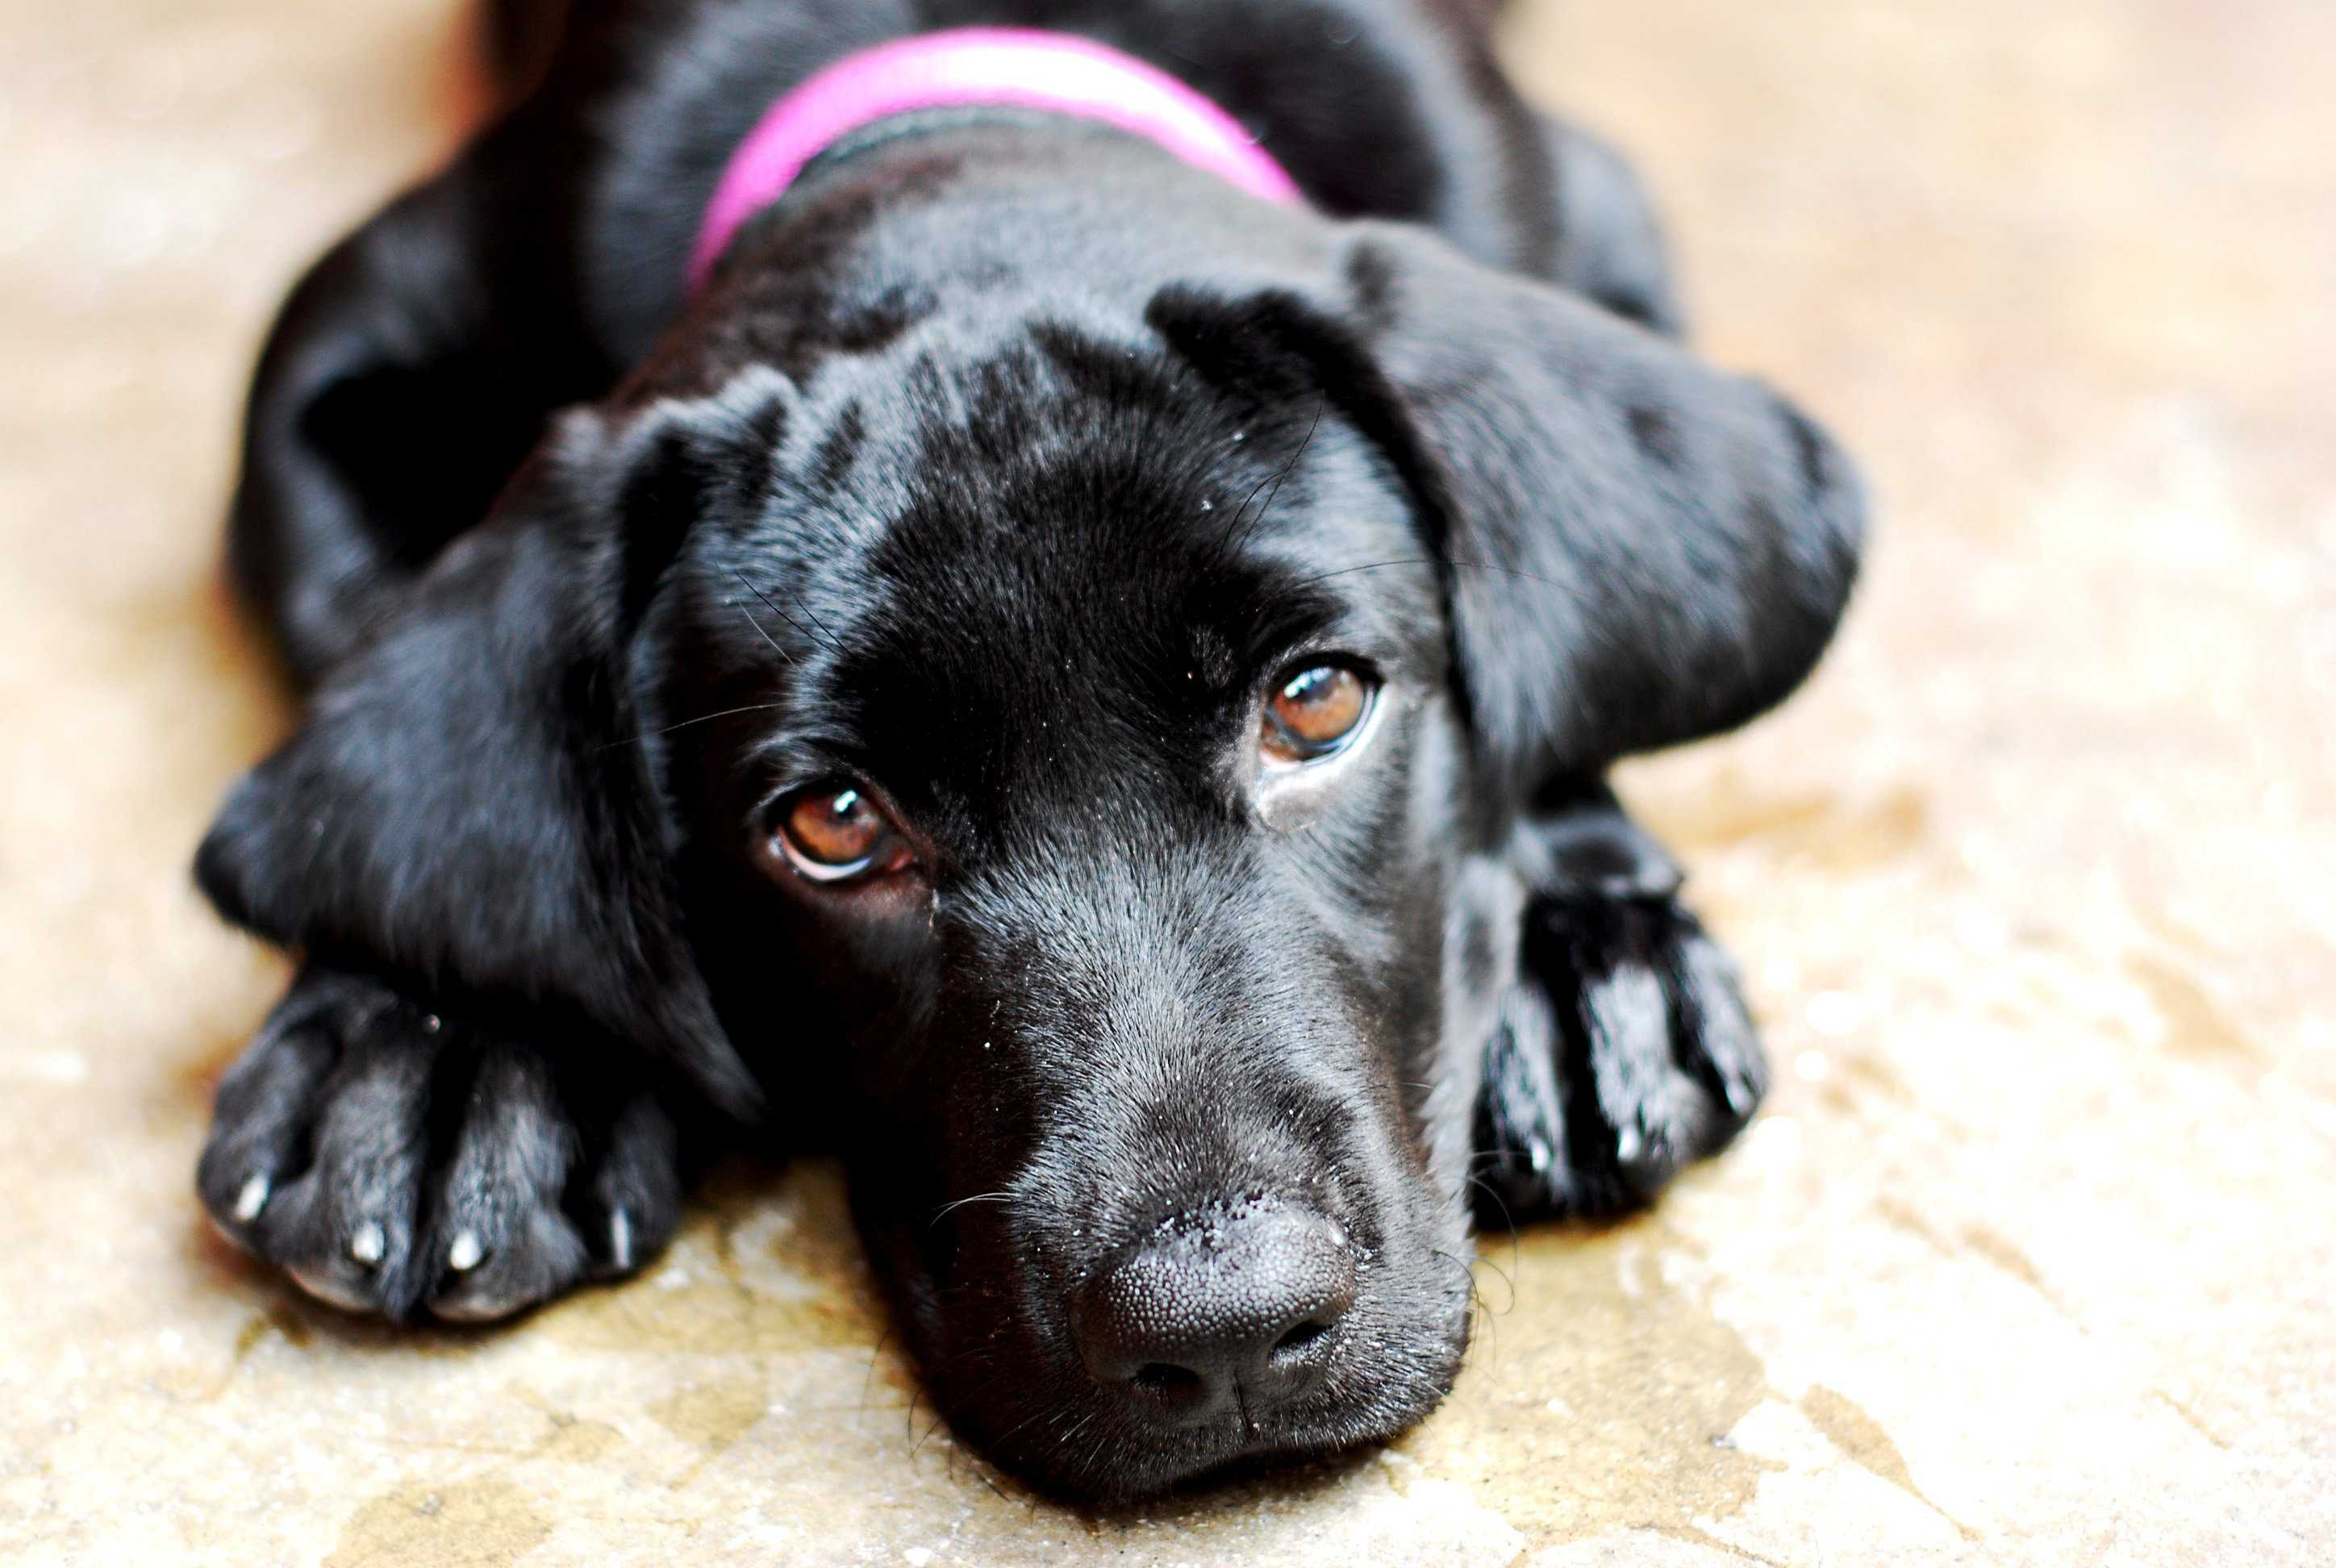
\includegraphics[width=\paperwidth]{images/dog.jpg}
    }
    \begin{frame}
    \end{frame}
}

% Cria um slide com uma única imagem, definida como imagem de fundo.
{%
    \usebackgroundtemplate{
        %\centering
        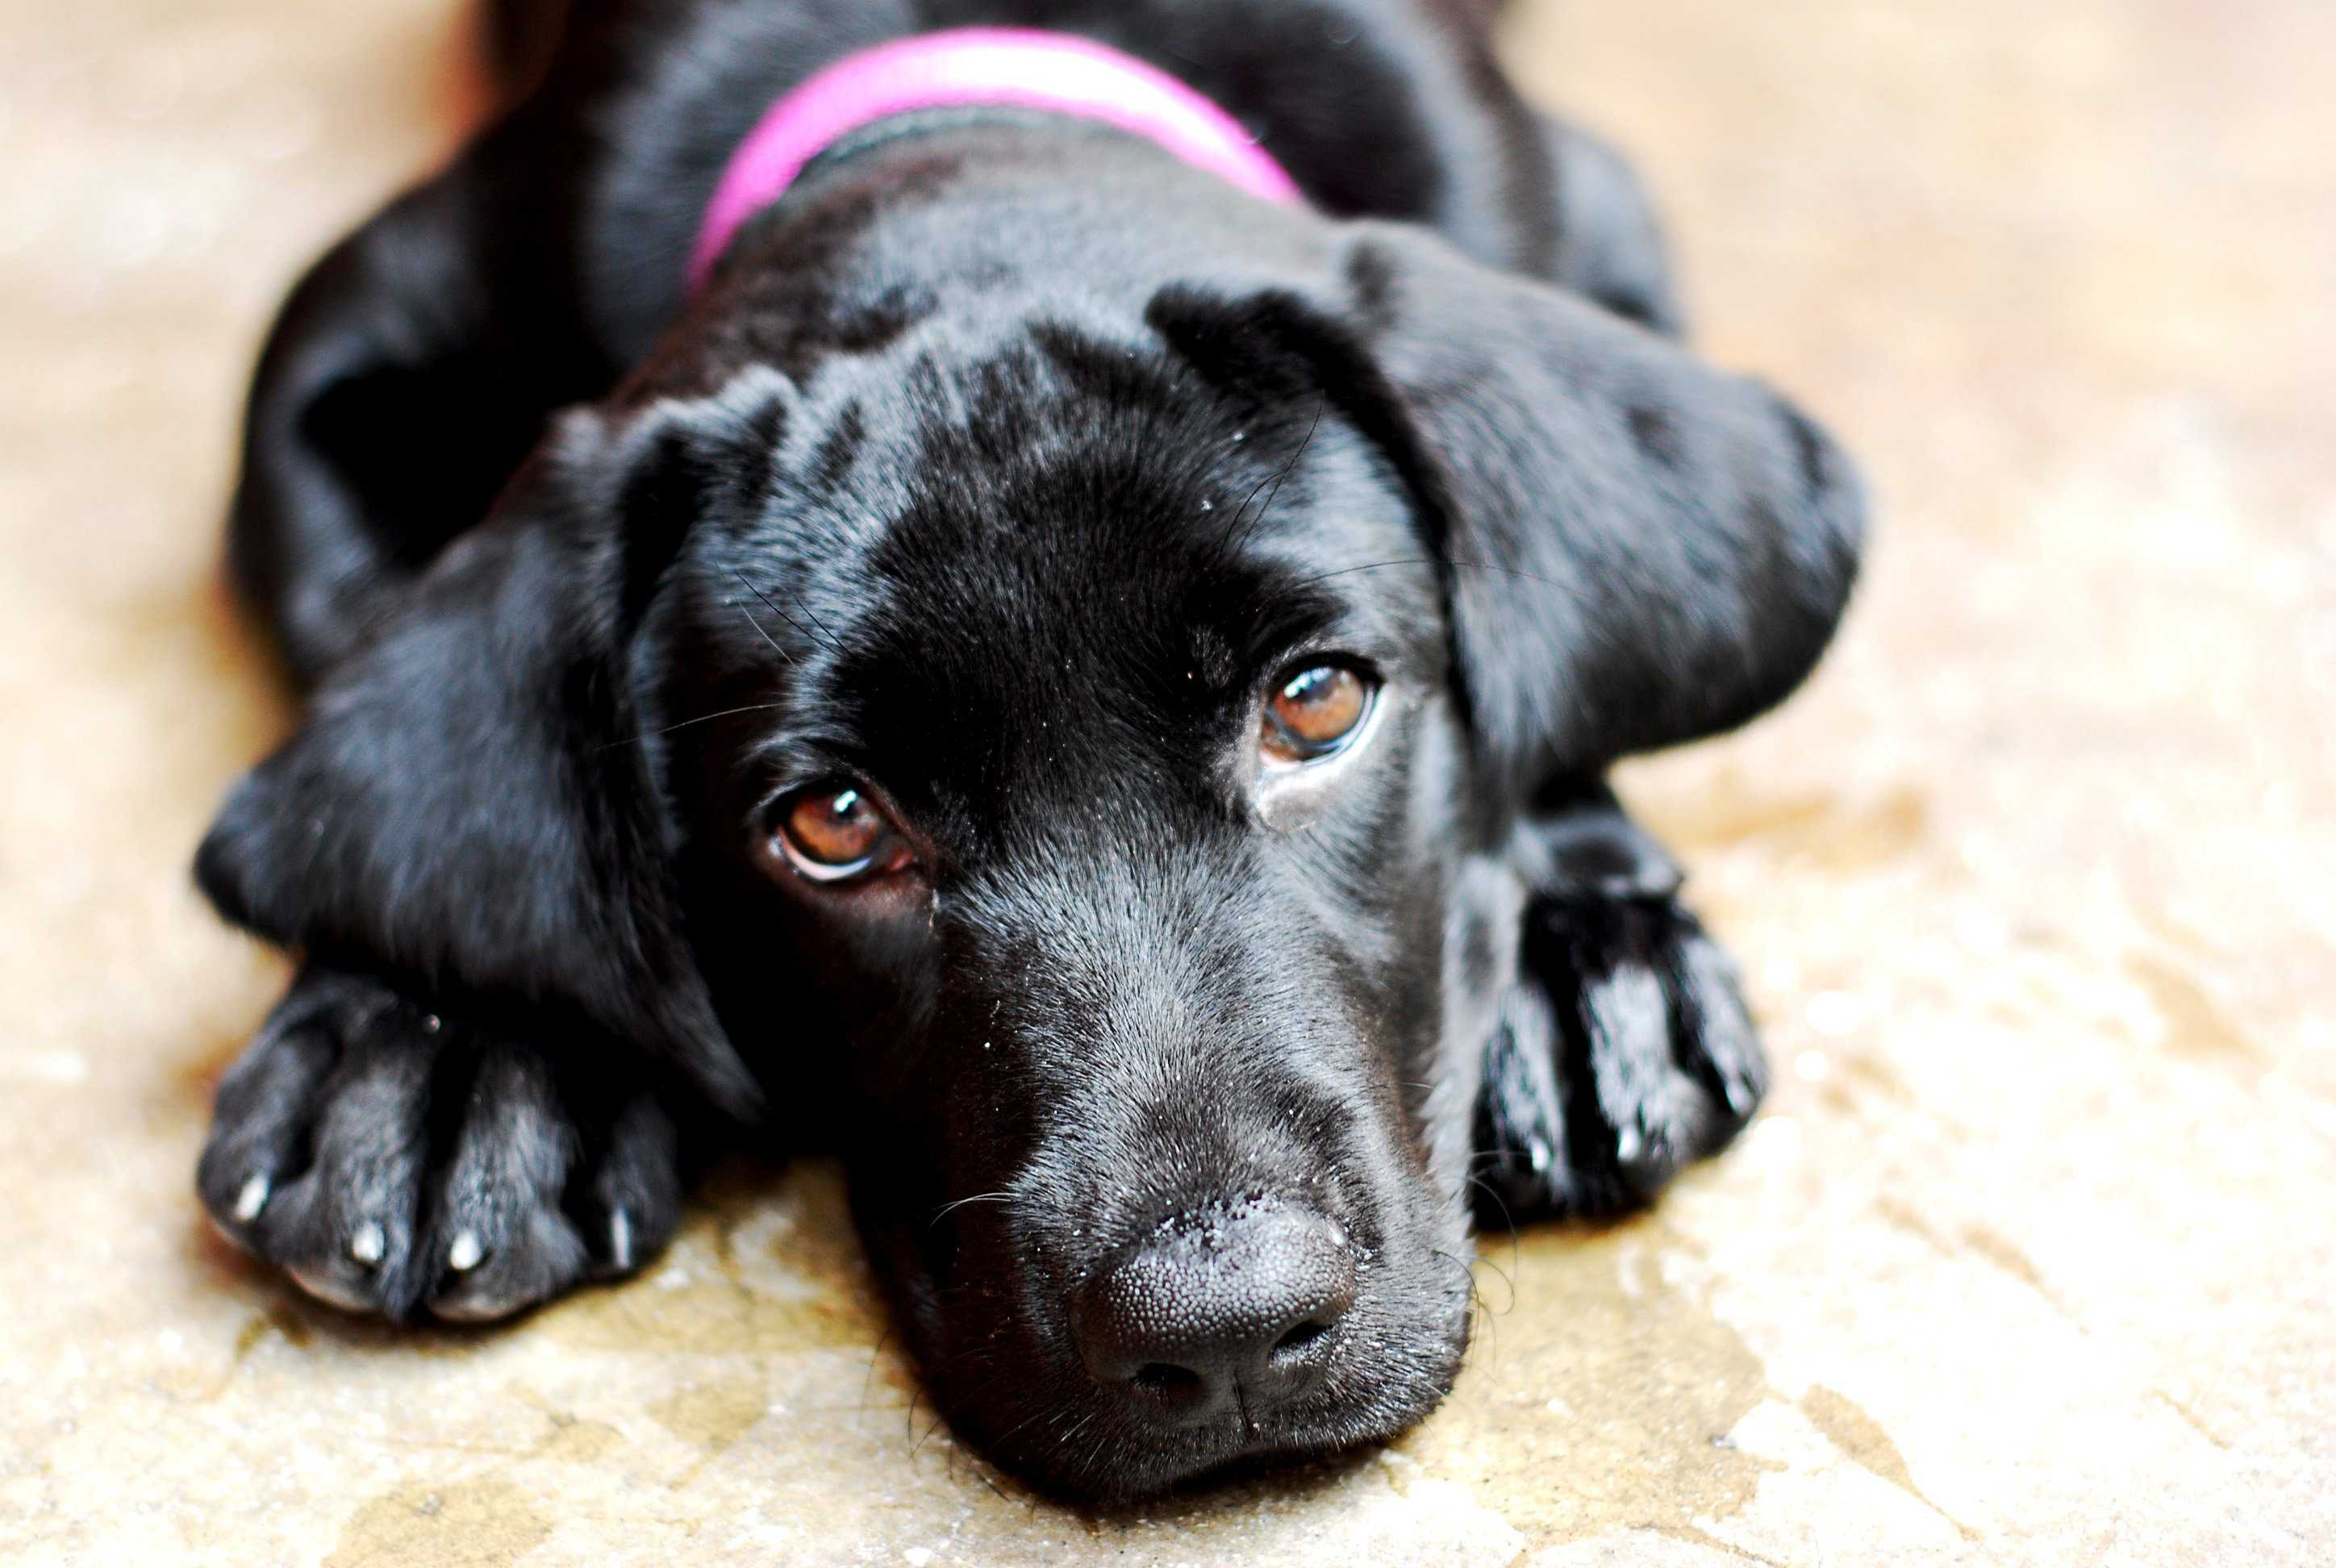
\includegraphics[width=\paperwidth]{images/dog.jpg}
    }
    \begin{frame}
        \begin{center}
        \vfill
        \vfill
        \color{white}
        \Huge \textbf{Got Linux?}
        \end{center}
        \vfill
        \vfill
        \vfill
        \vfill
        \vfill
        \hfill \tiny Ben Kranke/Getty
    \end{frame}
}

% Cria um slide com uma única imagem, definida como imagem de fundo.
% Creditos da imagem alinhados com Tikz
{%
    \usebackgroundtemplate{
        %\centering
        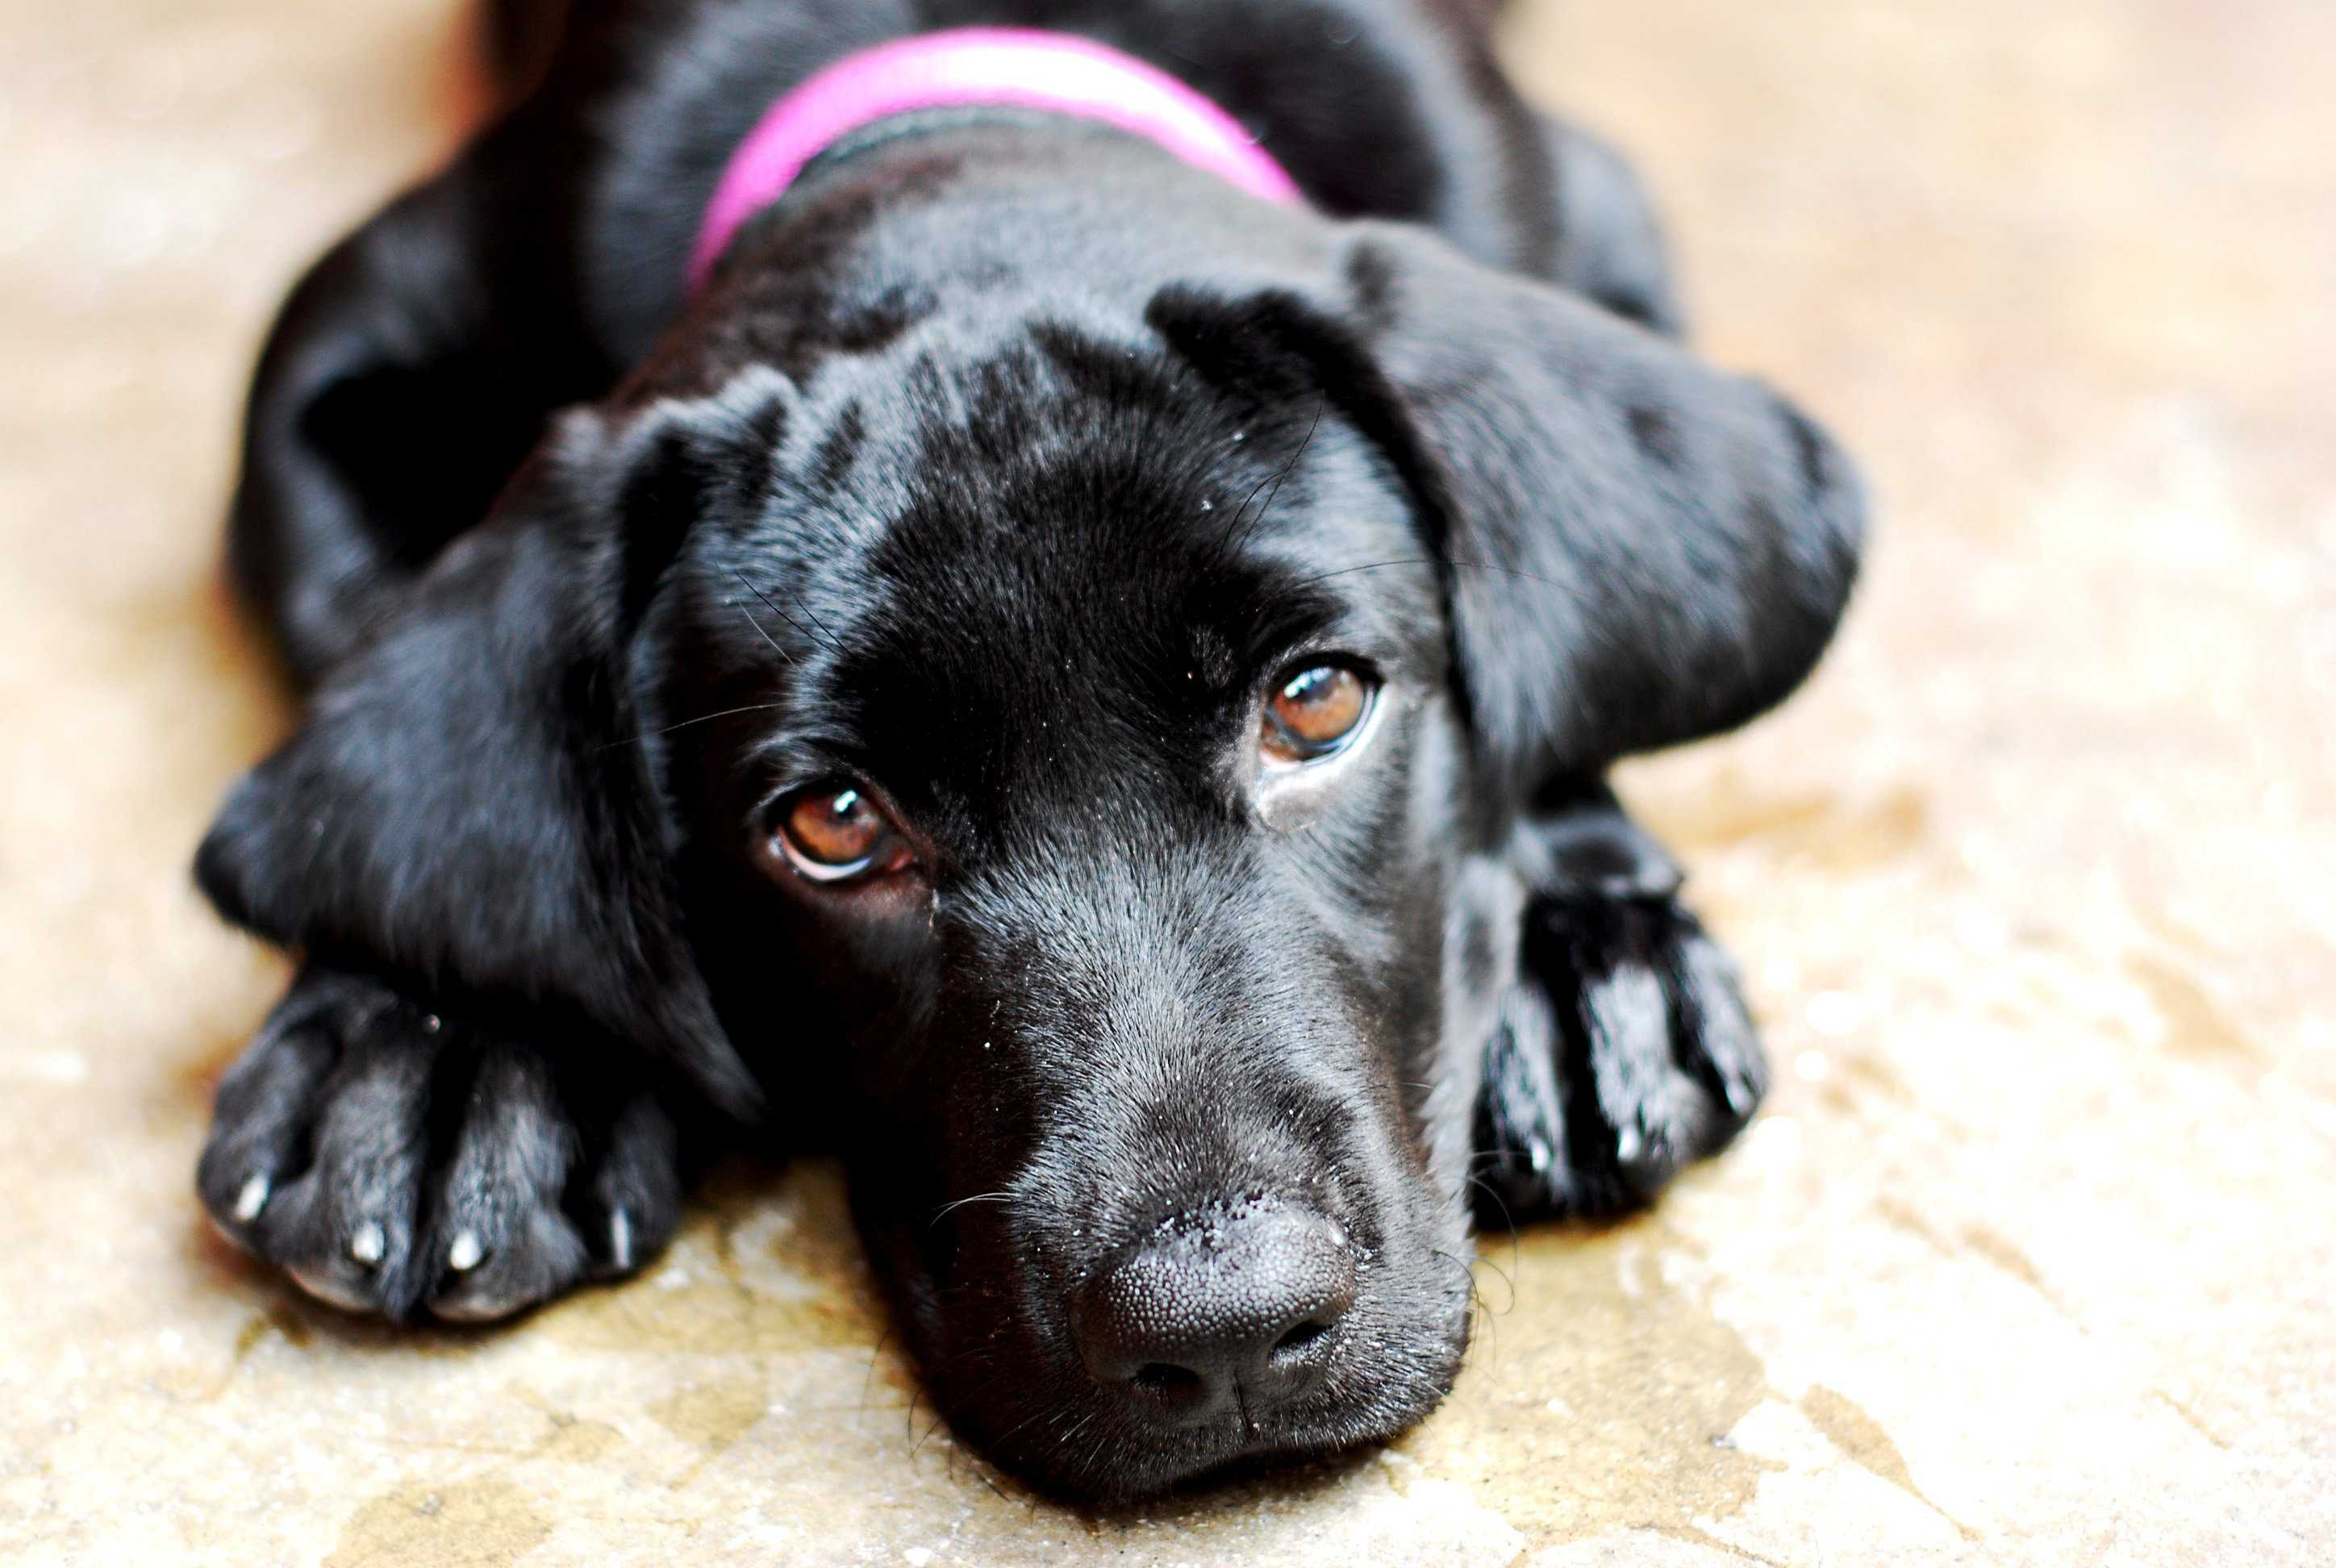
\includegraphics[width=\paperwidth]{images/dog.jpg}
    }
    \begin{frame}
        \begin{center}
        \color{white}
        \Huge \textbf{Got Linux?}
        \end{center}
        
    % Cria um overlay para uma imagem.
    \begin{tikzpicture}[remember picture,overlay]  
        % Posiciona o overlay na página
        \node [xshift=-2cm,yshift=1cm] at (current page.south east)
        % Adiciona o text, definindo seu tamanho
        {\tiny Ben Kranke/Getty};
    \end{tikzpicture}
    \end{frame}
}

% O pacote Tikz permite que se desenhe na página.
\begin{frame}
    \frametitle{Desenhando com Tikz}
    % Cria um overlay para uma imagem.
    \begin{tikzpicture}[domain=1:7,yscale=0.7,xscale=0.95]
    % Grid
    \draw[very thin,color=gray] (0.9,-0.1) grid (14,7);
    % eixo X
    \draw[->] (1,0) -- (14,0) node[right] {$x$}; 
    % eixo y
    \draw[->] (1,0) -- (1,7) node[above] {$f(x)$};
    
    % curvas
    \draw[color=red] plot(\x,\x) node[right,yshift=0.2cm] {\tiny $f(x) =x$};
    \draw[color=blue,domain=1:3.8] plot(\x,{\x*log2(\x)}) node[right] {\tiny $f(x) = x\lg x$}; 
    \draw[color=orange,domain=1:2.7] plot(\x,{\x*\x}) node[left] {\tiny$f(x) = x^2$};
    
    \draw[color=green,domain=1:14] plot(\x,{log2(\x)}) node[right] {\tiny$f(x) = \lg x$};

    \end{tikzpicture}
\end{frame}

\begin{frame}[t]
    \begin{center}
    \large Você pode alinhar o elementos com o topo.
    \end{center}
\end{frame}

\begin{frame}[b]
    \begin{center}
    \large Você pode alinhar o elementos com a parte de baixo.
    \end{center}
\end{frame}

\begin{frame}[c]
    \begin{center}
    \large Ou ao centro, que é o padrão.
    \end{center}
\end{frame}

\begin{frame}
    \frametitle{Para mais informações...}
    \begin{itemize}
        \setlength\itemsep{1em}
        \item{https://en.wikibooks.org/wiki/LaTeX/PGF/TikZ}
        \item{https://github.com/rafasgj/tchelinux-palestras.git \\ (tag poa-2017-5)}
    \end{itemize}
\end{frame}

\end{document}

